% # INFO:
% this file will produce a few warnings, even when working correctly:
% - using fallback Bibtex backend, cased because of the older backend, which may not support all features
% - Bad type area setting, caused by using a landscape page. The type area is malformed, but this is no problem if you only include external pages


% # choosing a document class:
% The command below is the first one you will see in pretty much any LaTeX document. It sets up the so called documentclass,
% which is what determines all of your styling and sets up loads of stuff for you. In general there are classes for pretty much
% every type of document you could need, but this project provides a few classes specialized for the Hochschule Hannover.
% You can find information about the classes and the options in the README, but here is an example setup with load of comments:
\documentclass[	%----------------------Preamble---------------------------------------------------%
		fontsize=11pt,  % fontsize
		a4paper,	    % papersize
		%twoside,		% double sided layout
		english,		% document language (also numberingsystem)
		%ngerman,		% document language (also numberingsystem)
		sans,			% font type (sans/roman)
		f1,				% HsH facultie (f1-f5)
		%draft			% quicker compilations, images are not included
	]{HsH-report}		% documentclass


% # the preamble:
% everything between `\docuemtnclass' and `\begin{document}' is called the preamble. Here you configure all settings for your document.
% The `\documentclass' command is actually part of that configuration. Lets see what you could do here:


% # packages
% To extend LaTeXes basic functionality, you can load additional packages. Some are already loaded, but others you load in as needed.
% Check the README about what's already loaded and what's recommended.
% Also, this classfiles automaticly check for a file called `config.tex', in which you can collect common configurations and reuse them across
% files in this and/or multiple projects. If you use the full template from GitLab, it provied a `config.tex' which only applies the settings,
% if the corresponding package is loaded, making it even more reusable.
%
% Here are some packages we are going to need with some explanations:
\usepackage{color}		% for colouring stuff
\usepackage{siunitx}	% units
\usepackage{listings}	% including formated code snippets
\usepackage{csvsimple}	% for importing CSV files
\usepackage{subfigure}	% for subfigures
\usepackage{soul}		% strikethrough text
\usepackage{amssymb}	% for spectial Math symbols
\usepackage{enumitem}	% more list options
\usepackage{lipsum}		% dummy text


% # bibliography
% While you can just create a super simple bibliography directly in your documents and format it completely yourself (see <https://en.wikibooks.org/wiki/LaTeX/Bibliography_Management#Embedded_system>)
% it is far more manageable and consistent to use a system called BibTeX, which allows you to maintain a file of all your sources and takes care of all
% the formatting for you. It also figures out which sources you use in your documents and only prints these, allowing for a single bibliography file
% you can use on multiple/all your projects. You can also create bibliographies on a chapter basis, if you prefer.
% To use it, just load the according package in your preamble, as shown below.
% Be aware that you need to run a separate program (`bibtex' or`biber') on your latex file for your citations to be rendered. But you usually don't
% need to run that every time.
% Also while this example is set up to use `bibtex' (because it is the default in loats of editors), the defaul for this project is the more modern
% `biber' command, so you need to change your editor accordingly if you omit the `backend=bibtex' option below:
\usepackage[backend=bibtex]{biblatex}

% now we load our bibliography file. Open it to see what it looks like
\addbibresource{bib/localBibliography.bib}


% # document information
% In your preamble you also list your documents information and metadata. These will be used on the title-page as well as being available throughout
% the document. Additionally, these documentclasses set up the resulting PDF file with the appropriate Metadata.
% You can just delety any of this comands or leave them empty if you don't need it for a project.
% See the following examples and what they create in the PDF file:
\author{
	Max Mustermann,
	Mira Musterfrau
} % the author and matrikelnr commands could also be on a single line, this is just more readable
\matrikelnr{
	1234567,
	9876543
}
\titlehead{Found on GitLab}
\subject{Example Project}
\title{How to write in Latex}
\subtitle{A helpful guide to get started and to show some common use cases}
\date{\st{01.01.2020}\\\today}
\professor{your Professor}
\keywords{some, informative, keywords}


% Now that you are all set, let's begin with the actual content of the document.
% Don't forget the corresponding `\end{document}'!
\begin{document} %----------- beginning of document -----------------------------------------------

% for longer documents it is custom to have different numbering until the first page of actuall content.
% For that use this command to switch to Roman pagenumbers and turn off chapternumbers:
\frontmatter

% While you can of course create your own title-page, either with latex or externally, the easiest way is to use the build in command.
% These classes redefine it to include the HsH-logo (depending on the chosen faculty) and to use the additional data provided in the preamble.
% You can also use the optional argument to change the title-pages alignment to l,c or r:
\maketitle[c]

% this command is provided by these documentclasses. It creates a standard Text at the bottom of the page and a line to sign on for every author.
% You are not restricted to this exact position and can use it where ever you want in your document, if you prefer it at the back, but it there.
\declarationAuthorship

% # abstract
% sometimes you are required to also create an abstract. Use this environment for that.
% It will create a new page and a heading for you as well as indenting the whole text block a little.
% if you have provided keywords, they will also be put at the end of the abstract.
\begin{abstract}
	\lipsum[5-6]
\end{abstract}

% This command will create the table of contents (TOC).
% Keep in mind, that LaTeX can only now about things it has already read. For everything that follows, it relies on temporary files which are created
% on the fly. So the complete TOC will only be rendered after at leas two LaTeX runs.
\tableofcontents

% the following command is the counterpiece of the `\frontmatter' command.
% It resets pagenumbers so that the next chapter is the first with actuall content.
\mainmatter


% now we can begin with the actuall relevant content. So let's beginn by creating the first chapter:
\chapter{What is LaTeX} \label{chap: latex}
	So you decided to get stated with LaTeX. Great! So let's talk a bit about the basic concept and differences it comes with.

	\medskip
	Up to this point you probably used a Word Processor like MS Word. The kind of workflow you know from there is often referred to as \emph{What you
	see is what you get}. You see the exact final layout as you type it, press some colourful buttons to insert stuff and if it doesn't want to do
	something you need, you're screwed.

	LaTeX on the other hand falls into the category of \emph{What you see is what you mean}, which describes all forms of markup languages. This means
	you create your LaTeX document as a simple plain text file without any from of formatting and mix in a bunch of commands telling what you mean.
	For example: "This is supposed to be a chapter heading", "make this bold" or "insert an image here". This source file will than be passed to a
	document processor (the LaTeX program), which will, depending on its settings, create the document for you. The advantage is, that you can use the
	same markup with all sorts of formattings and target file types.

	This is why working with LaTeX will require some getting used to and you will find yourself wanting to compile every five seconds to see the
	document update. Try to restrain yourself and concentrate on writing. You will find yourself working much faster.

	\section{Following this document}
		To see how the LaTeX source code and the resulting PDF correspond, I recommend you open this documents source code and PDF file next to each
		other and scroll through them simultaneously.

		If you already have a working LaTeX setup, most editors support \emph{SyncTex}, which allows you to jump between source code and PDF file and
		vice versa. You have to compile yourself, which will create a file called \lstinline{example.synctex.gz} in your project directory. Now you
		can \lstinline{<CTRL>+Click} in the PDF and the corresponding line of source code will be highlighted.

		The shortcut to jump from the source code into the PDF will depend on your Editor, but for VS Code its
		\lstinline{right Click}→\lstinline{SyncTex from cursor} or \lstinline{CTRL+ALT+J}.

	\section{Requirements to use LaTeX}
		As LaTeX files are just plain text file, you can edit them with any text editor (even windows notepad works, but that's just terrible).
		However, I would strongly recommend a more suitable editor. I use \href{https://code.visualstudio.com/}{Visual Studio Code} (which is a multi
		porpoise text editor that support all major programming languages) but you could also use something like
		\href{https://www.xm1math.net/texmaker/}{Texmaker}, which is an editor specifically for LaTeX. There is also the online editor
		\href{https://www.overleaf.com/}{Overfleaf}, which saves you the trouble of setting up your own LaTeX installation and provides everything you
		need in the cloud.

		\pagebreak\medskip
		As I have already mention above, you also need the LaTeX program. It comes bundled with packages and other additional software inside a
		Tex-distribution. There are two major ones, Texlive and MiKTeX. I recommend MiKTeX, but it essentially doesn't matter which one you choose.

		Once you have the distribution installed, test it by running \lstinline{pdflatex --version} in any terminal windows and it should return you
		some information about the installed version and setup.

	\section{Running LaTeX}
		To create a PDF file from your LaTeX source code, you can always navigate to the project folder in a terminal window and run
		\lstinline{pdflatex filename.tex}. However, if you have a decent editor installed, it will provide you with a button and do this for you.

		With these project files you also received a makefile, which demonstrates how to compile this example file successfully from the terminal. The
		README file also has some tips and information for you.

		If you use VS Code, this project also contains settings for LaTeX and recommended extensions. If you open the folder for the first time you
		will be asked if you want to install them and should than be able to compile this file.

	\section{LaTeX commands}
		Now lets look at the LaTeX command. Every one will begin with a \textbackslash\space followed by a letters only command name, like this:
		\lstinline|\command|. Most commands also accept input, which is put after it into curly brackets: \lstinline|\command{argument}|. They can
		accept multiple arguments either in multiple sets of curly brackets or as a comma separated list, depending on the command.

		Some commands also accept optional arguments. These are passed inside square brackets between the command name and the curly brackets, like
		this: \lstinline|\command[optional]{argument}|.

	\section{Getting more information}
		So what can you do if you get stuck or just want more information. The simple answer is: Google is your friend. Most questions have already
		been answered. For example on \href{https://tex.stackexchange.com/}{Tex Strackexchange}. Also, Overleaf has a great
		\href{https://www.overleaf.com/learn}{section for learning LaTex}.

		An of course you can always check the documentation, which you can find on \href{https://ctan.org/}{CTAN}.


\chapter{Basic text formatting} \label{chap: formating}

	To begin I want to show you the basics of how to get text onto the page and structure it. You can also see how I created this exact text as an
	example.

	\section{Headings} \label{sec: headings}
		The exact commands available will vary depending on you your documentclass, but they will always be a single command that excepts any text
		inside curly brackets, for example \lstinline|\section{text}|. The different commands form a hierarchy you can nest into each other, keeping
		track of its parent element. That means you don't have to worry about any formatting or numbering, LaTeX will handle that for you.

		When using an \emph{article} documentclass, the commands available are \lstinline|\section{}|, \lstinline|\subsection{}| and
		\lstinline|\subsubsection{}|. Should you need more nesting levels, you are usually overcomplicating things, but you could additionally use the
		\lstinline|\paragraph{}| command, which gives you a slightly bigger, bold first word for your paragraph.

		The \emph{report} documentclass adds the additional command \lstinline|\chapter{}| as the highest heading level. You can still use the previous
		three commands for the nested headings. A chapter automatically starts on a new page, so it should be at leas two pages long. You also get the
		command \lstinline|\part{}|, which creates a separate page for the part's title. These should only be used in very long documents.

	\section{Text paragraphs} \label{sec: paragraphs}
		Latex will format any text that is not part of a command (so not prefixes with a \lstinline|\| or inside \lstinline|{}|) as a plain-text
		paragraph. So the layout in your source code does not influence the layout of the resulting PDF. If you wanted to you could put everything on
		a single line, and it would work. This wouldn't be very readable however, so you should format your source code at leas a little. Putting
		every sentences on a new line is very common, or you can configure your editor to automatically break when the line gets to long (this is
		preconfigured if you open this project in VS Code).

		LaTeX will also automatically format your text to fill up all the available space and break long words for you. Sometimes, if you use special
		words LaTeX doesn't know, you may need to tell it where to split those. For one off cases you can just put \lstinline|\-| where you want a
		break and for words you use a lot you can declare the hyphenation in the preamble as a space separated list, for example like this:
		\lstinline|\hyphenation{word list donau-dampf-schiff}|

		Lots of online sources will list the double-backslash (\lstinline|\\|) as the command for a line break. While this is not wrong, you should
		not use it to break your text. Instead, you should use \lstinline|\par| to denote the end of a paragraph. As programmers are lazy, LaTeX will
		actually insert this command for you, if you just leave an empty line between to blocks of text. Using the correct command allows LaTeX to
		better find automatic breakpoints, allows you to define the spacing between paragraph and has some other benefits.

	\section{Text spacing} \label{sec: spacing}
		By default, these classes add no spacing between paragraph, but sometimes you want to visually enforce a breakpoint in your argumentation. For
		that you can add some space in between to paragraph by using one of the commands \lstinline|\bigskip|, \lstinline|\medskip| or
		\lstinline|\smallskip|. How much space you want depends on your tase, but you should keep it consistent. Here is an example:

		\bigskip
		This text has a big space before it,

		\medskip
		Here I used just some medium spacing

		\smallskip
		and this is a small space.

	\section{Breaking pages} \label{sec: pagebreak}
		Sometimes you will find yourself in situations, where you don't like where LaTeX splits your text to the next page. So first, take some
		advice: Don't worry about it for now. Your text will probably change a few times before its final. Just leave it.

		If you are at the final stage, you can do a beautifying pass. Now you can use \lstinline|\pagebreak| to tell LaTeX about better places to
		break the text.

		Should you still not be happy (this happens especially with multiple images/tables in close proximity) you most likely have to little text and
		should redesign your document. But if you absolutely want to print it that way, you can use \lstinline|\clearpage| to force all
		figures/tables to be put onto the page and then start a new page.

	\section{Text styling} \label{sec: styling}
		When writing text, you will need to \emph{emphasize} certain parts of the text. The easiest way is to use the \lstinline|\emph{}| command
		around you text. You can also nest it \emph{to \emph{emphasize} even more}.

		If you want to change to a specific font-type, you can do that like this:

		\smallskip
		\begin{tabular}{l l}
			\lstinline|\underline{text}| & \underline{Underlined} \\
			\lstinline|\textbf{text}| & \textbf{Bold Font} \\
			\lstinline|\textii{text}| & \textit{Italic Font} \\
			\lstinline|\textrm{text}| & \textrm{Roman Font} \\
			\lstinline|\texttt{text}| & \texttt{Typewriter Font} \\
			\lstinline|\textsc{text}| & \texttt{Small Caps Font} \\
		\end{tabular}

		\medskip
		You might also want to change your text colour, which is what the \lstinline{color} package is for. It provides the
		\lstinline|textcolor{colour}{text}| command, \textcolor{red}{which allows you} \textcolor{blue}{to change your text colour}.

	\pagebreak
	\section{Special characters} \label{sec: special-charaters}

		\subsection{LaTeX command characters}
			As in most programming languages, some characters are used for LaTeXes commands and can't be used in text directly. Here is a table
			explaining them all:

			\smallskip
			\begin{tabular}{l l l}
				\emph{character} & \emph{special meaning} & \emph{how to get character} \\
				\textbackslash & beginning of a command & \lstinline|\textbackslash| \\
				\{ and \} & denote a code block & \lstinline|\{| and \lstinline|\}|\\
				\% & beginning of a comment & \lstinline|\%| \\
				\# & macro parameter character & \lstinline|\#| \\
				\$ & beginning/end of math mode & \lstinline|\$| \\
				\textasciitilde & non-breaking space & \lstinline|\textasciitilde| \\
				\emph{only inside math mode:} \\
				$\_$ & subscript & \lstinline|\_| \\
				\textasciicircum & superscript & \lstinline|\textasciicircum| \\
			\end{tabular}

		\subsection{Invisible characters}
			To properly typeset your text you may need a number of special characters under specific circumstances:

			\smallskip
			\begin{tabular}{l l l}
				\emph{explanation} & \emph{command} & \emph{example} \\
				non-breaking space & \lstinline|~| & Max~Mustermann (Names shouldn't be broken) \\
				3/4 non-breaking space & \lstinline|\;| & 10\;000 (separate thousands)\\
				medium non-breaking space & \lstinline|\:| & z.\:B. (abbreviations) \\
				1/2 non-breaking space & \lstinline|\,| & 1\,V (number + unit) \\
				normal space & \lstinline|\space| & in case some command eats up all your space \\
			\end{tabular}


\chapter{Examples} \label{chap: one}
	{\color{red}red text} and {\color{blue}blue text} \\
	different subscripts: \normalsubscripts$R_t$ \upsubscripts$R_t$ \\
	using Units: $R=200\,\mohm + \SI{0.34567453}{\volt\per\metre} - 5\,\si{\second\per\metre\squared}$ \\
	some information\cite{laboranleitung:physik}\\
	german number: $3,5$ english number: $3.5$\\ % note changes when using ngerman document option


	\section{Using formulas} \label{sec: formula}
		a numberd formula:
		\begin{equation}
			\label{eq: einhalb} % always lable your stuff
			0,5=\frac{1}{3}
		\end{equation}
		\autoref{eq: einhalb} is nice, but how about multiple lines:
		\begin{equation}
		\begin{split} % you need do nest this
			x &= x^2+3 \\
			\Leftrightarrow 0 &= x^2-x+3 \\
		\end{split}
		\end{equation}
		and how could you align formulas?
		\begin{align}
			x_1 &= 6 &&|\;\mbox{mit } x \in \mathbb{N} \\
			x_2 &= 33+\abs{\frac{1}{4}} &&|\;x_1+3 \\
				&= 33,25 &&\mbox{| don't number everything} \notag \\
			x_3 &= 10^{22}
		\end{align}


	\section{using Units}
		For this the \lstinline{siunitx} package is used. It provides Macros for all units.
		\begin{equation}
			200\,\kg
		\end{equation}
		The space between a number and it's unit should be a protected half-space, which can be created in latex using \lstinline{\,} In the classfile
		siunits is set up to use a separate macro for each subunit, even for size-modifiers:
		\begin{equation}
			200\,\mm \cdot 2\,\volt
		\end{equation}
		Siunits also allows for reformatting of numbers as well as units. Use the \lstinline{\SI} and \lstinline{\si} macros for that:
		\begin{equation}
			e = \SI{1.602176634E-19}{\coulomb} % formats number + units, autospacing, transform to german comma
		\end{equation}
		\begin{equation}
			\SI[exponent-to-prefix]{1e-6}{\metre}% you can also autocalculate prefixes
		\end{equation}
		\begin{equation}
			124\,\si[per-mode=fraction]{\kilo\metre\per\second\squared} % only units
		\end{equation}
		\begin{equation}
			\num{0.0004}\,\lumen % only numbers,  \per and \squared do not work
		\end{equation}


	\section{using images}
		Images can just be imported and used in a float environment with a caption and a lable to reference it. (see \autoref{fig: random image})
		\begin{figure}
			
\includegraphics[width=.6\textwidth]{img/lorem-ipsum.jpg}
			\caption{just a random image}
			\label{fig: random image}
		\end{figure}\\
		You can also display two or more images together, using the \lstinline{subfigure} package. You can also resize or crop Images, as seen in
		\autoref{fig: resize} and \autoref{fig: croped}
		\begin{figure}
			\subfigure[a smaller Version]{\label{fig: resize}
\includegraphics[scale=0.1]{img/lorem-ipsum.jpg}}
			\subfigure[a croped image]{\label{fig: croped}
\includegraphics[width=.4\textwidth, trim=5cm 0 5cm 0,clip]{img/lorem-ipsum.jpg}}
			\caption{some more images}
		\end{figure}

		Plots can be created directly with latex. It is recommended to do this in subfiles and just import the finished PDF pages. This speed us
		compilertimes by a lot. You should not change the size of precompiled images to keep fontsizes consistent.
		\begin{figure}
			\includegraphics[page=2]{plt/examplePlot.pdf}
			\caption[centering]{a nice plot}
			\label{fig: plot1}
		\end{figure}
		\begin{figure}
			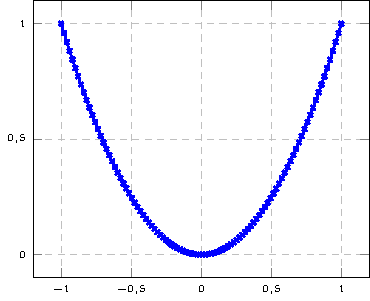
\includegraphics[page=1]{plt/examplePlot.pdf}
			\caption{a area plot}
			\label{fig: area}
		\end{figure}

		\pagebreak
		Circuit diagramms can also be created using a package called \lstinline{circuitikz}. It is also recommended to get familiar with Inkscape which
		has a very good export to latex feature, as you can see in \autoref{subfig: svg}. If you use Inkscape, there is a list of all electrical
		symbols \href{https://de.wikipedia.org/wiki/Liste_der_Schaltzeichen_(Elektrik/Elektronik)}{here on wikipedia}. You can downlload them as
		\lstinline{.svg} files (not as png!) and just drag\&drop them into Inkscape.
		\begin{figure}
			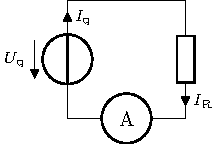
\includegraphics{crc/exampleCircuit.pdf}
			\label{subfig: circuit}
			\caption{a circuit diagramm}
		\end{figure}

		\pagebreak
		Using Inkscape, you can create SVG-vector graphics and import them easily into Latex.
		\begin{figure}
			\def\svgwidth{0.3\textwidth} % define desired width
			\graphicspath{{svg/}} % Inkludepath needet for the inputed file, double curly brackets needed for unknown reason
			\input{svg/exampleSVG.pdf_tex} % input the Latexfile generated by inkscape
			\caption{A image created with Inkscape}
			\label{subfig: svg}
		\end{figure}
		\enlargethispage{4\baselineskip}

	\section{using tables}
		Tables are a little bit complicated in LaTex, but don't worry, here are some examples:
		\begin{table}
			\caption{a simple table}
			\label{tab: table 1}
			\begin{tabular}{r|l}
				A & B \\\hline\hline
				1 & 2 \\\hline
				3 & 4 \\\hline
			\end{tabular}
		\end{table}\\
		As you can see, tables are build using two nested environments. The \lstinline{table} creates a floate just like a \lstinline{figure} would.
		You can then just give it a caption and a lable.\\
		The \lstinline{tabular} environment creates the actual table. You need to devine the alignment for every column and give delimiters between
		lines. Each cell is ended by a \& and a newline is created as always. Using \lstinline{\hline} creates a vertical line after the row.\\
		Here is a more complex example:
		\begin{table}
			\caption{a bigger table}
			\begin{tabular}{r|c|r l|l}
				ID & NAME & Price & Currency & Stock \\\hline
				1 & Product A & 10 & EUR & 20 \\
				2 & Stuff & 1 & USD & 200 \\
				\multicolumn{2}{c|}{A cool Teddy} & 50 & EUR & 1\\\hline
			\end{tabular}
		\end{table}


	\section{lists and enumerations}
		This is a nested List:
		\begin{itemize}
			\item hallo
			\begin{itemize}
				\item temp
				\begin{itemize}
					\item temp
					\begin{itemize}
						\item temp
					\end{itemize}
				\end{itemize}
			\end{itemize}
		\end{itemize}

		\pagebreak
		And this is a nice checklist:
		\begin{checklist}
			\item first
			\item urgent
			\begin{checklist}
				\item sub item
				\item and another
			\end{checklist}
			\item continue
		\end{checklist}



	\section{CSV files}
		\label{sec: messwerte}
		import a csv as table:
		\par % a par is needed before the autotabulat since the kernel update from 01.06.21
		\csvautotabular{csv/bsp.csv}\\

		or do it manually to get more control:
		\begin{table}
			\caption{a nice list of numbers}
			\begin{tabular}{c|c}
				first row & second row \\\hline\hline
				\csvreader[
					late after line=\\\hline,
					late after last line=\\\hline
				]{csv/bsp.csv}{}{number: $\csvcoli\,\metre$ & is not \csvcoliii}
			\end{tabular}
		\end{table}


\section{formating code} \label{sec: code}
	use the listings package:
	% gobble removes the whitespace that is only in the latex code to make it look organised
	\begin{lstlisting}[language=c,gobble=8]
		#include <stdlib.h>
		#include <sdtio.h>

		int main(void) {
			printf("Hello World");
			return 0;
		}
	\end{lstlisting}
	% or input from external file:
	%\lstinputlisting[language=c]{main.c}

\chapter{seperating the document}
	This was inputed from anothe file!!
	\vspace{4em}\\
	It can be usefull to seperate yout document into chapterfiles. This allows to only compile  the changed parts of the document or work with
	multiple people at the same time, but on different chapters.\\
	If you use a more advanced text editor like VS-Code, the editor even compiles the hole document, even when you are editin a subfile.

\clearpage
\KOMAoptions{paper=landscape,pagesize,DIV=9} % rotate page to landscape mode (because why not XD), this causes a warning, use with cation
\recalctypearea
\chapter{attachment}
% manually include a PDF as not numbered section
\textbf{\Large{Messprotokoll oder so}} % just so it'S not empty
\phantomsection % Anker für den Hyperlink
\addcontentsline{toc}{section}{Messprotokoll} % add to table of content
\chaptermark{Messprotokoll}	% change headmark
%\includepdf[pages=-,pagecommand={},width=\paperwidth]{temp.pdf} % comment in to include pdf
As you can see its also possible to have some pages sideways. Just keep in mind you might need to adapt the margins

\newpage
\KOMAoptions{paper=portrait,pagesize} % and back
\recalctypearea

\printbibliography
\noindent\begin{minipage}{\textwidth} % prevent automatic pagebreaks
	\listoffigures
	\listoftables
\end{minipage}
\end{document}
